\chapter{Realisierung}\label{real}
Mit dem in Kapitel~\ref{basics:ifc} vorgestellten \textit{IFC Standard} existiert ein umfangreiches Framework zur Beschreibung sämtlicher für die Baubranche relevanter Daten. 
Im Zusammenspiel mit dem darauf aufbauenden \textit{Building Information Modeling} wird ein einheitliches Verwaltungskonzept für das Planen, Bauen und Bewirtschaften von Infrastruktur vorgeschlagen (siehe Kapitel~\ref{basics:bim}).
Darum stellen im IFC Format vorliegende Gebäudepläne den Ausgangspunkt dieser Arbeit dar.

\section{Modellierung}\label{real:modellierung}
Dank den in Kapitel~\ref{basics:ifcopenshell} vorgestellten Open-Source-Projekten zu den Technologien \textit{IFC} und \textit{BIM} sowie deren Anbindungen an die ebenfalls öffentliche 3D-Grafiksoftware Blender (siehe Kapitel~\ref{basics:blender}) ist es möglich auf einen komplett kostenlosen Technologiestack zur Modellierung von Gebäuden im IFC Format zurückzugreifen.
Die Option Blender mithilfe sogenannter \textit{Add-ons} an spezielle Projekt-abhängige Anforderungen anzupassen, macht diese Modellierungsumgebung noch zweckdienlicher.
Ein solches Add-on ist zum Beispiel \textit{blenderbim} (siehe Abschnitt~\ref{basics:blenderbim}). 
Dieses ermöglicht es ein IFC Projekt direkt in Blender entweder neu zu beginnen oder ein Vorhandenes zu bearbeiten.
Für diese Arbeit relevant ist zunächst das Erstellen und Annotieren von Wänden beziehungsweise Wandtypen, sowie das Anbringen von Öffnungen.
Beide Konzepte sind Teil des IFC Standards und wurden bereits ausführlich in Kapitel~\ref{basics:ifc} vorgestellt.
Blenderbim ermöglicht es in wenigen Schritten einen neuen \textit{IfcWallType} zu definieren und daraus \textit{IfcWall} Objekte zu erstellen.
Diese können mit den von Blender nativ angebotenen Werkzeugen angepasst werden.
Zusätzlich gibt es weitere hilfreiche, von Blenderbim eingeführte Modellierungsmöglichkeiten.
Dank der Möglichkeit eigene \textit{IfcPropertySets} (siehe Kapitel~\ref{basics:ifc_properties}) zu definieren, lassen sich die in Kapitel~\ref{concept:raster} konzeptionierten Raster- und Modulinformationen zu den neu definierten Wandtypen hinzufügen.
Bei Generierung eines \textit{IfcWall} Objekts werden diese Properties ebenfalls an das neue Wandstück geknüpft.
Damit können diese Informationen sowohl an das nachfolgende Wall Detailing übermittelt, als auch zur intuitiveren Modellierung des 3D Modells herangezogen werden, indem man Nutzern durch ein für diese Arbeit entwickeltes Add-on das für jeden Wandtyp zugeordnete Raster bei sämtlichen Transformationsvorgängen aufzwingt (siehe Abschnitt~\ref{concept:raster}).
Dadurch werden kleine Modellierungsfehler von vornherein vermieden.

\section{Wall Detailing}
In Abschnitt~\ref{concept:wall_detailing} wurde das Wall Detailing als der Vorgang, ein als geometrischer Körper definiertes Wandstück in ein konkretes Mauerwerk zu überführen, bezeichnet.
Innerhalb des IFC Standards werden einige mathematische/geometrische Repräsentationen der sogenannten \textit{IfcWall} unterstützt, um neben einfachen Boxen auch komplexere Formen abbilden zu können.
Beispielsweise ist es möglich in das Modell eines Hauses zunehmend dünner werdende Wandstücke, kurvige Wandstücke oder Wandstücke, welche nur durch ein arbiträres Vieleck beschrieben werden können zu integrieren.
Standardmäßig haben \textit{IfcWalls} aber einen einfachen Quader als Grundform, was für die Fallstudien dieser Arbeit ausreichend ist.
Die Unterkapitel dieses Abschnitts folgen den in Kapitel~\ref{concept:wall_detailing} genannten Schritten, um von einer Menge solcher Wände hin zu einer Menge an Bausteinen zu gelangen, die den gewünschten Mauerwerksverband darauf anwenden.

\subsection{Konvertieren und Filtern der Daten der IFC Datei}
Den ersten Schritt stellt das Extrahieren aller notwendigen Daten aus dem vorliegenden IFC Modell dar.
Für die Fallstudien dieser Arbeit sind sowohl alle Objekte des Typs \textit{IfcWall} als auch die daran angeknüpften Objekte vom Typ \textit{IfcOpeningElement} (siehe~\ref{basics:IfcOpeningElement}) von Interesse.
Diese entstehen während der Modellierungsphase etwa durch Anbringen von Fenstern oder Türen an einer Wand.
Zusätzlich werden aus den in den \textit{IfcPropertySets} der Wandstücke hinterlegten Daten Informationen über das zu verwendende Modul und Raster ausgelesen.
Mithilfe der Werkzeuge der in Kapitel~\ref{basics} vorgestellten Python Bibliothek \textit{IfcOpenShell} (siehe~\ref{basics:ifcopenshell}) ist dies in wenigen Schritten möglich.
\begin{figure}[htb]
  \centering
  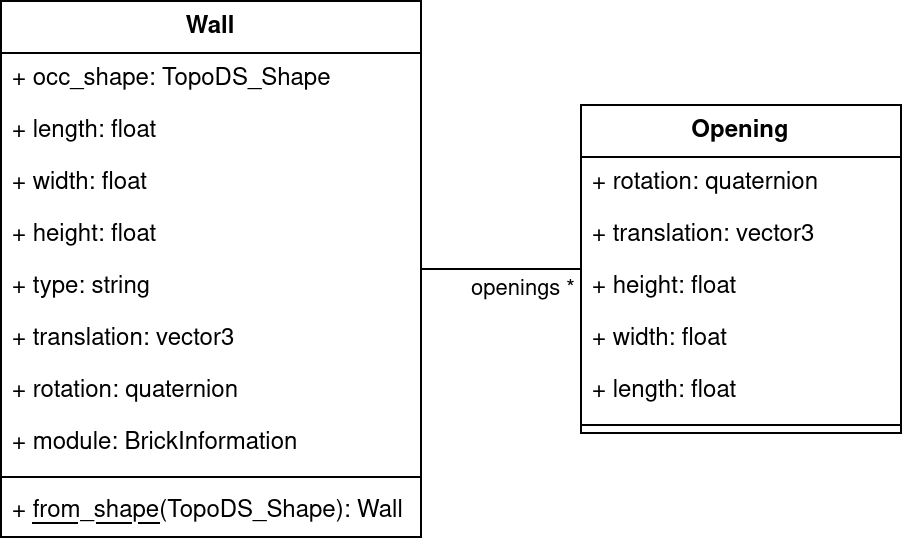
\includegraphics[width=0.65\columnwidth]{fig/klassendiagramm_ifc_to_wall.drawio.png}
  \caption{Klassendiagramm von der Klasse \textit{Wall} und der Klasse \textit{Opening}.}\label{fig:real:ifc_to_wall}
\end{figure}

Zunächst werden aus jeder \textit{IfcWall} ein Objekt der Klasse \textit{Wall} erzeugt und anschließend mit deren in der IFC Datei angegebenen Öffnungen (Opening) versehen.
Deren Zusammenspiel in dieser Arbeit kann dem Klassendiagramm aus Abbildung~\ref{fig:real:ifc_to_wall} entnommen werden und ist eine vereinfachte Version der Struktur innerhalb des IFC Modells.
Um die globalen Transformationen der \textit{IfcWalls} und \textit{IfcOpenings} zu errechnen, muss der in Abbildung~\ref{fig:IfcWall_Hierarchie} gezeigten Klassenhierarchie nach oben gefolgt werden, da die in den Kindern eines Objekts angegebene Transformation relativ zu dessen Eltern angegeben ist.
Im Anschluss werden die nun globalen Transformationen der Openings wiederum in eine relative Transformation zum davon betroffenen Wall-Objekt umgewandelt.
Das erleichtert später die Berechnungen für das Anwenden der Öffnungen in einer Wand.
Da sich diese Arbeit zunächst ausschließlich mit quaderförmigen Wandstücken beschäftigt, müssen alle zuvor aus dem IFC Modell extrahierten Wandstücke auf diese Eigenschaft geprüft werden.
Alle anders geformten \textit{IfcWalls} werden in dieser Arbeit zunächst ignoriert.
Somit ist gewährleistet, dass lediglich passende Wandstücke an die nachfolgenden Schritte weitergegeben werden.

\subsection{Anwenden des Moduls}
Mit dem zu jedem Wandstück festgelegten Modul werden nun alle Wandstücke in Schichten aufgeteilt.
Diese Schichten werden von der Klasse \textit{WallLayer} in Abbildung~\ref{fig:real:apply_module} repräsentiert und durch eine Instanz der Klasse \textit{WallLayerGroup} gruppiert.
Deren Höhe entspricht im Normalfall der Höhe des jeweiligen Moduls.
Lediglich die oberste Schicht kann durch falsch modellierte Wandstücke eine niedrigere Schichthöhe aufweisen.
Dies ist der Fall, wenn die Gesamthöhe des Wandstücks nicht exakt einem Vielfachen der Höhe des Moduls entspricht und ein nicht aufzuteilender Rest existiert.
Das Aufteilen in Schichten erleichtert es im Anschluss Berechnungen an Wandstücken durchzuführen und Beziehungen zwischen ihnen zu finden.
\begin{figure}[tbh]
  \centering
  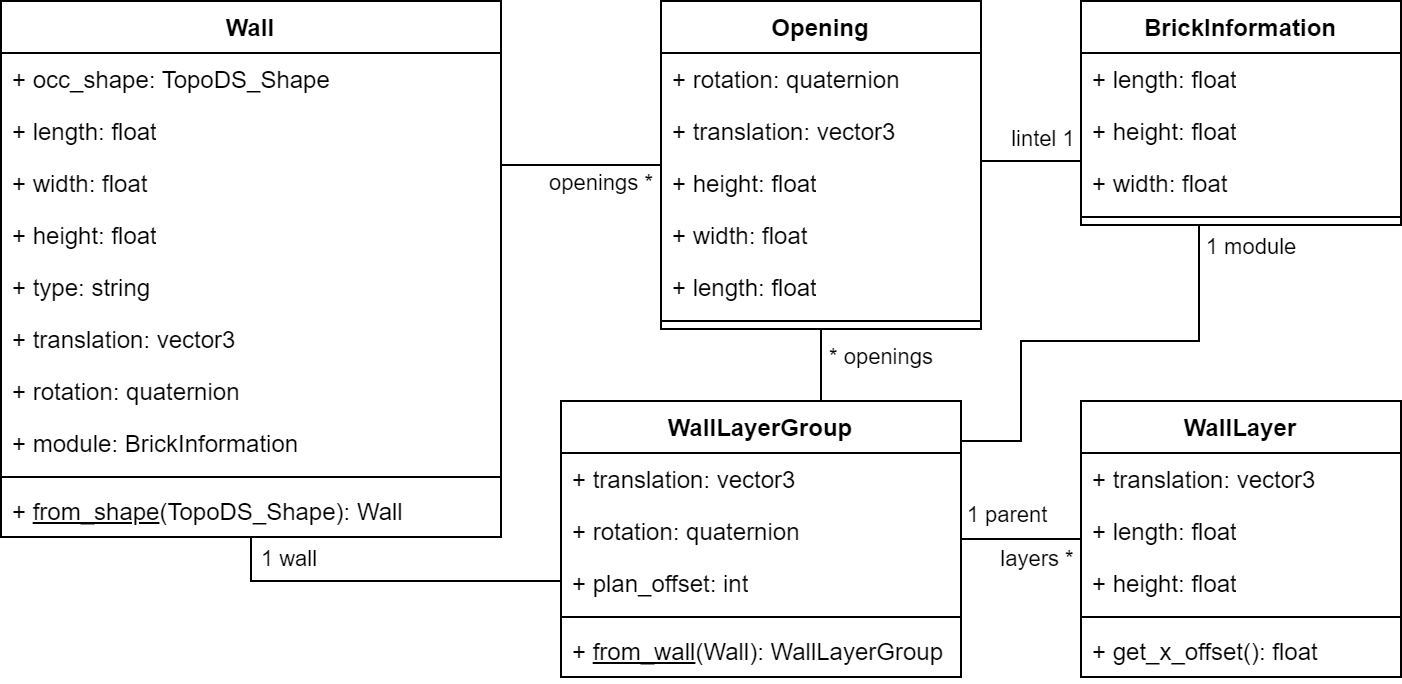
\includegraphics[width=0.8\columnwidth]{fig/klassendiagramm_apply_module.drawio.png}
  \caption{Klassendiagramm nach Anwenden des Moduls.}\label{fig:real:apply_module}
\end{figure}

\subsection{Kombinieren passender Wandstücke}\label{real:combination}
Eine solche Beziehung stellen Wände dar, die, wie bereits in Kapitel~\ref{concept:relations_wandtuecke} definiert, durch mehrere einzelne Objekte modelliert wurden, eigentlich aber eine Einheit bilden.
Daher werden in diesem Schritt alle Wandstücke miteinander verglichen und eventuell kombiniert, sodass jeweils ein gefundenes Paar durch ein einzelnes Wandstück repräsentiert wird.
Um zwei Wandstücke zu sinnvoll kombinieren zu können, müssen die Eigenschaften aus Kapitel~\ref{concept:combination_properties} gelten.
Allerdings kann Punkt~\ref{concept:schichten}, welcher Berührung oder Überlappung voraussetzt, mittlerweile wie folgt verschärft werden:

\begin{enumerate}
\setcounter{enumi}{4}
\item\label{real:schichten} Mindestens eine Schicht des einen Wandstücks berührt, überlappt oder befindet sich exakt eine Modulhöhe ober- oder unterhalb einer Schicht des anderen Wandstücks.
\end{enumerate}

In Abbildung~\ref{fig:concept:combination_example_base} treten verschiedene Konstellationen von Wandstücken auf, die miteinander kombiniert werden müssen.
Das aus Wandstück 1 und 2 gebildete Paar erfüllt alle oben genannten Eigenschaften und weist eine Teil-Überlappung auf.
Somit müssen beide Wandstücke miteinander kombiniert werden.
Den obersten Bereich füllen sowohl Wandstück 5 als auch Wandstück 6, sodass dort eine komplette Überlappung vorliegt.
Auch diese beiden Wandstücke werden kombiniert, wobei dabei im Prinzip einfach eines verworfen wird.
Zusätzlich muss dieser Bereich, wie auch Wandstück 7, mit Wandstück 2 kombiniert werden, da die beiden Paare sich an Ober- und Unterkante berühren.
Einen weiteren Fall stellen seitliche, nicht überlappende Berührungen dar, wie sie zwischen Wandstück 2 und 3 zu sehen ist.
Auch für dieses Paar sind alle Voraussetzungen zur Fusion erfüllt.
Lediglich Wandstück 4 muss nicht mit dem Rest vereint werden, da dafür kein Paar existiert, das die obigen Eigenschaften erfüllt.
Anhand von Abbildung~\ref{fig:real:combination_example_solution_xoffset} kann man erkennen, dass Wandstück 4 im weiteren Verlauf des Detailings tatsächlich unabhängig betrachtet werden kann. 

Während dem Kombinieren von zwei Wänden wird ein Wandstück schichtweise in das Andere überführt.
Dabei werden alle Schichten paarweise miteinander verglichen, um diejenigen Paare zu finden, die die Eigenschaften aus Punkt~\ref{real:schichten} erfüllen.
Ein solches Paar wird dann wie folgt miteinander verschmolzen:
\begin{enumerate}
  \item Errechne die kleinste und die größte relative x Koordinate der linken und rechten Ecken beider Schichten.
  \item Die Differenz der beiden Werte entspricht der neuen Länge der resultierenden Schicht.
  \item\label{real:comb_tmp_point} Die kleinste x Koordinate ist deren neue linke Eckkoordinate.
  \item Mit dieser Eckkoordinate aus Punkt~\ref{real:comb_tmp_point} und der halben neuen Länge kann nun der Mittelpunkt der resultierenden Schicht berechnet werden. Dieser entspricht der relativen Translation einer Schicht in Abhängigkeit der dazugehörigen \textit{WallLayerGroup}.
\end{enumerate}
\begin{figure}[htb]
  \centering
  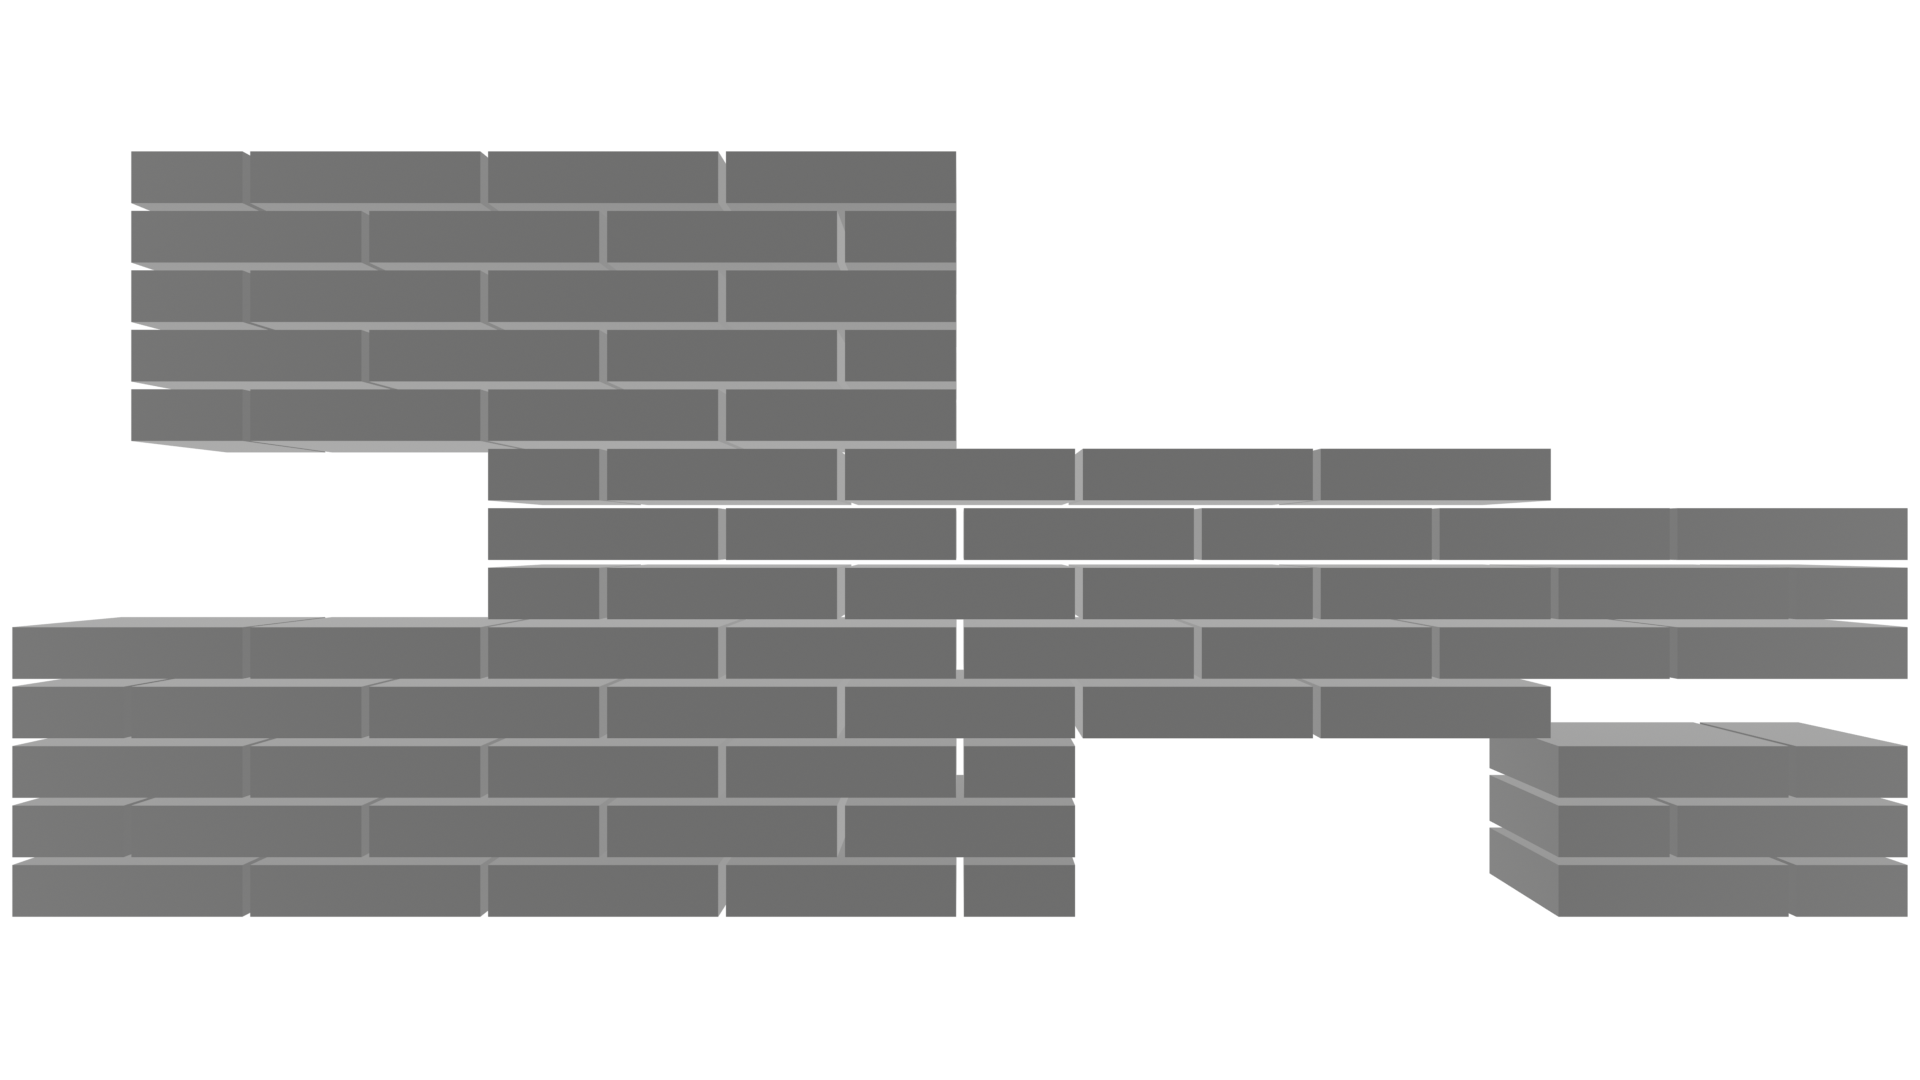
\includegraphics[width=0.8\columnwidth]{fig/Real_Combination_Output.png}
  \caption{Ergebnis mit berücksichtigtem \textit{x\_offset}.}\label{fig:real:combination_example_solution_xoffset}
\end{figure}

\begin{figure}[hbt]
  \centering
  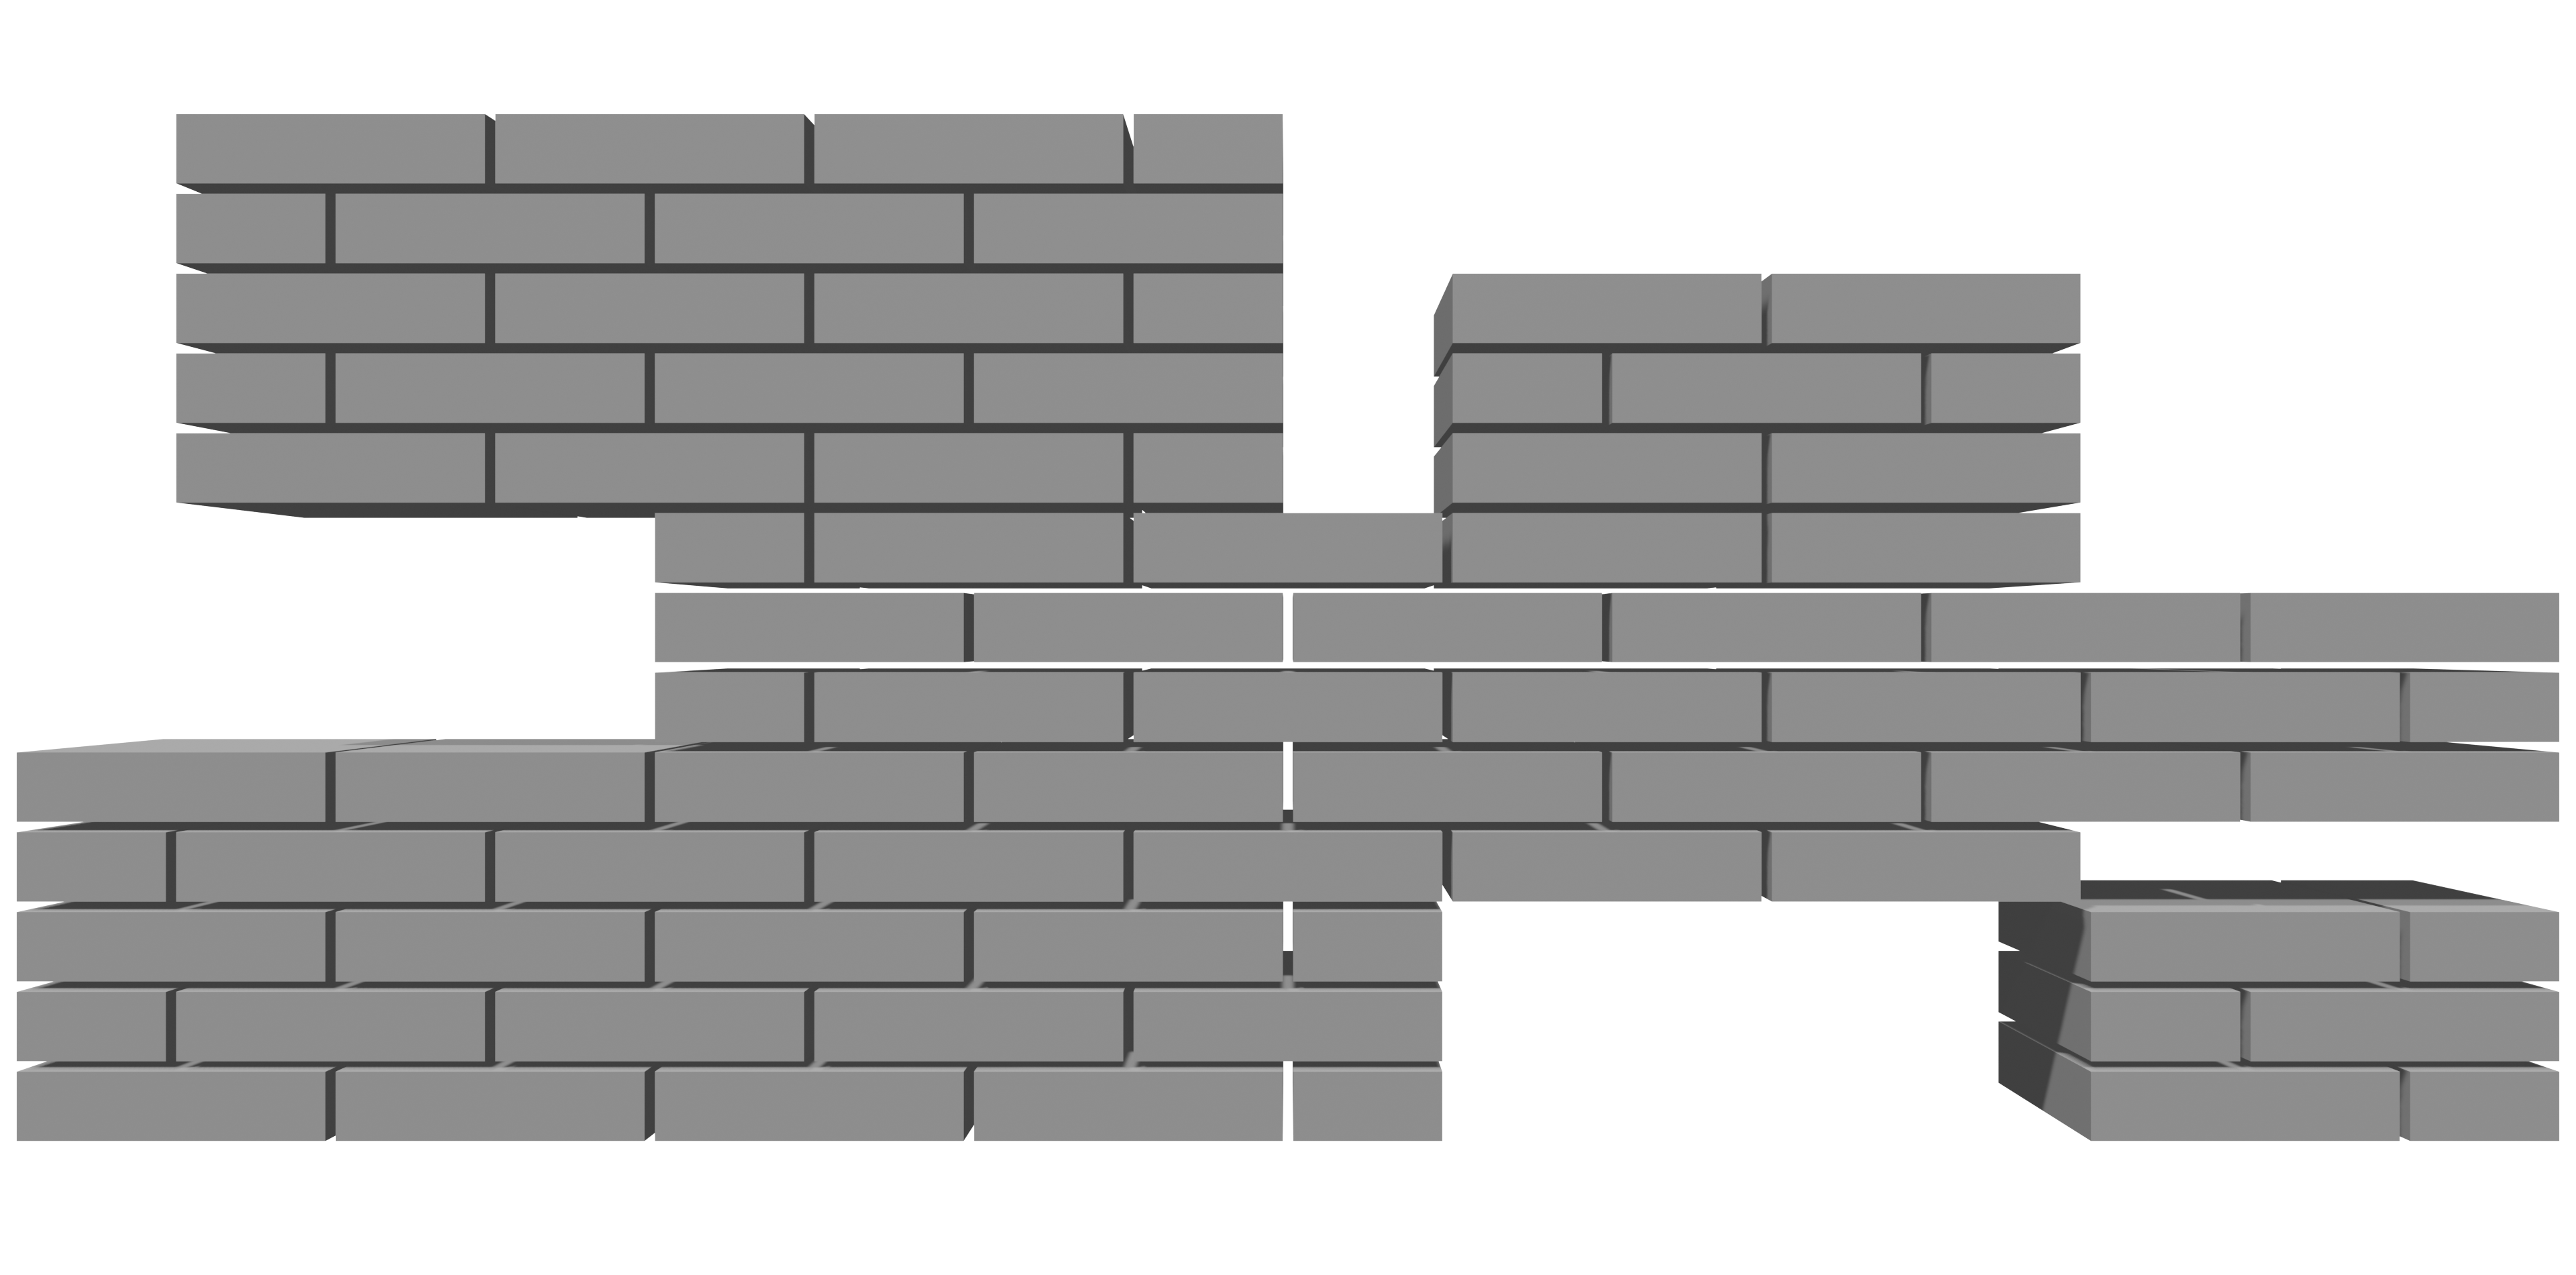
\includegraphics[width=0.8\columnwidth]{fig/Real_Combination_Output_No_XOffset.png}
  \caption{Ergebnis mit ignoriertem \textit{x\_offset}.}\label{fig:real:combination_example_solution_no_xoffset}
\end{figure}

Steht ein Wandstück in X-Richtung versetzt auf einem anderem, so ist es notwendig diesen Versatz während dem nachfolgenden Detailing zu berücksichtigen.
Ignoriert man dies, kann das, durch Verletzung des vorgeschriebenen Überbindemaßes (siehe Abschnitt~\ref{basics:Mauerwerksverband}), zu den in Abbildung~\ref{fig:real:combination_example_solution_no_xoffset} gezeigten Fehlern innerhalb des Mauerwerksverbands führen (zum Beispiel zwischen Wandstück 2 und 7).
Dieser, nachfolgend als \textit{x\_offset} bezeichnete Versatz ist definiert als die Differenz zwischen der kleinsten lokalen X-Koordinate aller Schichten eines Wandstückes (mittlerweile repräsentiert durch eine \textit{WallLayerGroup}) und der lokalen X-Koordinate der zu betrachtenden Schicht.
Der daraus resultierende Wert wird später dazu verwendet den anzuwendenden Mauerwerksverband erst an passender Stelle zu beginnen.
Dadurch erzielt man einen einheitlichen Verband über das gesamte Wandstück und verhindert den in Abbildung~\ref{fig:real:combination_example_solution_no_xoffset} gezeigten Fehlerfall.
Eine weitere Eigenschaft, die aus dem Kombinieren mehrerer Wandstücke entstehen kann, ist das Vorhandensein unterbrochener Schichten oder, anders ausgedrückt, mehrerer Schichten auf einer Höhe innerhalb des resultierenden Wandstückes.
Dies ist ebenfalls in Abbildung~\ref{fig:concept:combination_example_base} zu sehen. 
Zwischen drei Schichten des Bereichs der Wandstücke 5 und 6 und des Wandstücks 7 ist eine Lücke.
Durch das Einbeziehen des \textit{x\_offset} können derartige Situationen jedoch ebenfalls gelöst werden, da für jedes Teilstück einer Schicht ein eigener \textit{x\_offset} berechnet wird.
Nach Vereinigung aller passenden Paare reduziert sich die Zahl der ursprünglichen Wandstücke aus dem Modell in Abbildung~\ref{fig:concept:combination_example_base} von sieben auf zwei.
Die korrekte Durchführung mit angewandtem \textit{x\_offset} ist in Abbildung~\ref{fig:real:combination_example_solution_xoffset} zu sehen.

\subsection{Finden und Lösen von Beziehungen}\label{real:find_and_solve}
Nun wird die aus dem vorherigen Schritt entstandene neue Menge an Wandstücken auf weitere Beziehungen untersucht.
Für das Wall Detailing relevante Beziehungen stellen Ecken, T-Kreuzungen und X-Kreuzungen dar (siehe Kapitel~\ref{concept:solving_beziehungen}).
Der Grund dafür ist die Komplexität in diesen Bereichen die vorgeschriebenen Normen einzuhalten.
Dazu zählt zum Beispiel das in Abschnitt~\ref{basics:Mauerwerksverband} genannte Überbindemaß.
In Abschnitt~\ref{concept:corner_etc_properties} wurden bereits die Eigenschaften aufgeführt, mithilfe derer sich die gesuchten Beziehungen identifizieren lassen.
Wichtige Informationen für jede dieser Beziehungen sind einerseits die Punkte, an denen sie sich im Raum befinden, andererseits die Art der Beziehung (also die Unterscheidung zwischen Ecke, T- oder X-Kreuzung).
Die Position ist der Schnittpunkt der Richtungsvektoren beider Wandstücke entlang ihrer lokalen X-Achsen.
Die Unterscheidung der Beziehungen kann mithilfe des Vorgehens, das ebenfalls in Abschnitt~\ref{concept:corner_etc_properties} erläutert wurde, durchgeführt werden.
Dabei spielen die Anzahl der Wandstücke, die sich in einem Punkt schneiden und der Ort des Punktes innerhalb der beteiligten Wandstücke eine Rolle.
Da ein Wandstück zu diesem Zeitpunkt schon als Menge an Schichten vorliegt, wird das Verfahren, wie es bereits oben getan wurde, paarweise auf alle Schichten angewandt.
Somit werden für jede, sich durch Verkettungen über mehrere Wandstücke erstreckende Schicht alle Kreuzungs- und Eckbereiche ausfindig gemacht.
Bevor aber eine neue Eckinstanz angelegt wird, muss überprüft werden, ob an dem errechneten Schnittpunkt bereits ein Eckbereich gefunden wurde.
Falls dem so ist, kann die dazugehörige und bereits vorhandene Eckinstanz lediglich um die Schichten des neuen Paares erweitert werden.
Dadurch kann im selben Schritt bereits die Zuweisung der Art der Beziehung vorgenommen werden.
Durch die Eckinstanzen werden nun die bis dahin unabhängigen Wandstücke, welche durch den vorherigen Schritt bereits schichtweise und kombiniert vorliegen, miteinander verknüpft.
\begin{figure}[h!]
  \centering
  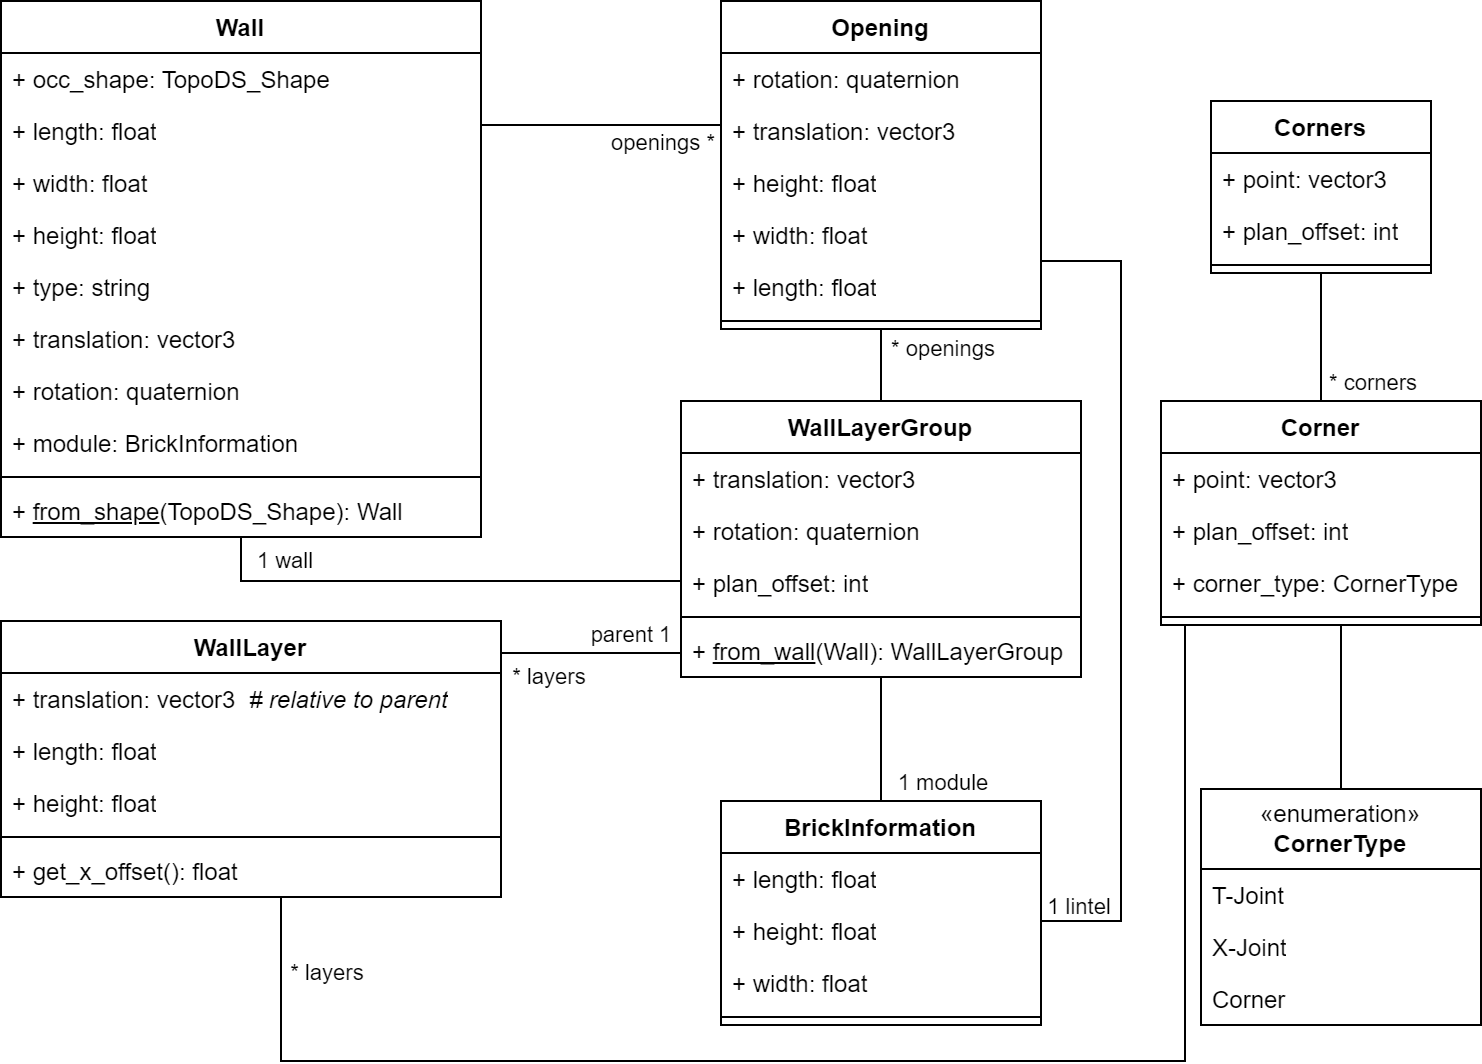
\includegraphics[width=0.8\columnwidth]{fig/klassendiagramm_corners.drawio.png}
  \caption{Klassendiagramm nach Errechnen der Eckbereiche.}\label{fig:real:class_diagram_corners}
\end{figure}
Ein nützlicher Nebeneffekt der schichtweisen Betrachtung der Eckbereiche ist, dass nun auch zwei Wände mit unterschiedlichen Höhen, die gemeinsam einen Eckbereich bilden, korrekt dargestellt werden können, denn es werden nur für die Schichten Eckinstanzen erzeugt, die in beiden Wandstücken vorhanden sind.
Die daraus resultierende neue Datenstruktur ist im Klassendiagramm in Abbildung~\ref{fig:real:class_diagram_corners} zu sehen.
Objekte der Klasse \textit{Corner} (bisher als Eckinstanzen bezeichnet) halten alle notwendigen Informationen zu jedem gefunden Eckbereich einer Schicht, während ein Objekt der Klasse \textit{Corners} dafür zuständig ist, die wachsende Liste an Eckinstanzen auf geteilte Schnittpunkte zu überprüfen.
Wird eine Eckinstanz an einer schon vorhandenen Position im Raum in die Liste eingefügt, so wird der dort bereits liegende Eckbereich lediglich um die neuen \textit{WallLayer} erweitert und falls nötig, dessen \textit{CornerType} angepasst.
Wie bereits erwähnt werden dabei die Voraussetzungen aus Kapitel~\ref{concept:corner_etc_properties} zur Unterscheidung der \textit{CornerTypes} herangezogen.

\subsection*{Lösen der Beziehungen}
In Abschnitt~\ref{concept:solving_beziehungen} wurde die Problematik der Eckbereiche bereits ausführlich behandelt.
Je nach gewählten Verband und anzuwendenden Modul können unterschiedliche Problemzonen beim Setzen der Bausteine auftreten.
Das Ziel dieses Schritts ist es, die jeweiligen Eck- oder Kreuzungspläne der betroffenen Wandstücke so anzuordnen, dass die dazwischenliegenden Wandbereiche unter Einhaltung des festgelegten Mauerwerksverbands lückenlos aufgefüllt werden können.
Dies ist nur möglich, wenn die Längen der modellierten Wandstücke zum gewählten Verband passen.
Unter der Annahme ein Modell ist mit den ausgewählten Modulen und Mauerwerksverbänden lückenlos baubar, führt das in Abschnitt~\ref{concept:solving_beziehungen} vorgestellte Vorgehen zu einer Lösung. 
Dabei werden die sogenannten \textit{plan\_offsets} so manipuliert, bis eine lückenlose Lösung gefunden wurde.
Sowohl Eckbereiche (siehe Klasse \textit{Corner} im Klassendiagramm aus Abbildung~\ref{fig:real:class_diagram_corners}) als auch die Wandstücke (mit der Klasse \textit{WallLayerGroup} realisiert) besitzen dieses Attribut.
Diese \textit{plan\_offsets} geben an, mit welchem Index des angegebenen Eck- oder Wandstückplans in der untersten Schicht einer \textit{WallLayerGroup} beim Berechnen der konkreten Bausteine begonnen werden muss.

Das in dieser Arbeit angewandte Verfahren stellt derzeit lediglich eine Verbesserung der Exhautionsmethode dar.
In Kapitel~\ref{concept:solving_beziehungen} wurde bereits festgestellt, dass alle durch mindestens einen \textit{Corner} verbundenen \textit{WallLayerGroups} verkettet zusammenhängen.
Daraus ergibt sich ein Abhängigkeitsgraph, der im Normalfall sämtliche Wandstücke eines Gebäudemodells miteinander verbindet.
Durch Festlegen des \textit{plan\_offset} eines einzigen Eckbereichs, können alle direkt und indirekt damit verbundenen Wandstücke und Eckbereiche daran angepasst werden.
Denn ändert man den \textit{plan\_offset} eines Eckbereichs, müssen alle darüber und darunterliegenden \textit{Corner} ebenfalls angepasst werden, um die vorgeschriebene Reihenfolge des Planes weiterhin einzuhalten.
Auch die Distanz, die ein Eckbereich in die daran anschließenden geraden Schichten ragt, kann sich dadurch verändern.
Dies ist anhand des Beispiels in Abbildung~\ref{fig:concept:loesen_von_beziehungen1} nachvollziehbar.
Je nach Eckplankonfiguration sind die weißen Reste jeder Schicht unterschiedlich groß.
Darum muss auch die \textit{length} (ebenfalls Teil des Klassendiagramms in Abbildung~\ref{fig:real:class_diagram_corners}) jeder Verbindungsschicht aller darüber und darunterliegenden \textit{Corner} neu berechnet werden.

Das Anpassen eines geraden Reststücks an einen damit verbundenen \textit{Corner} ist eine von zwei Operationen, die der Lösungsalgorithmus anwenden muss.
Die Zweite ist das umgekehrte Anpassen eines \textit{Corners} an ein bereits angepasstes gerades Reststück.
Bei beiden Operationen werden diejenigen \textit{plan\_offsets} aller Schichten der Ecke beziehungsweise des Wandstücks gesucht, die zu einer lückenlosen Lösung führen, ohne die Reihenfolge der Pläne zu verletzen.
Die Startkonfiguration des Verfahrens ist lediglich ein Knoten des Abhängigkeitsgraphen und ein daran angewandter \textit{plan\_offset}.
Davon ausgehend können diese Operationen abwechselnd auf die nächsten Nachbarknoten und die dazwischenliegenden Wandstücke angewendet werden, bis alle Knoten des Graphen abgearbeitet wurden.
Findet sich mit einer Startkonfiguration keine valide Lösung, so wird eine neue gewählt; entweder durch Verändern des \textit{plan\_offsets} oder dem Auswählen eines neuen Startknotens.
So gibt es je nach Komplexität eines Modells immer noch einen großen Lösungsraum, dieser wurde aber mithilfe des Abhängigkeitsgraphen deutlich minimiert, da das Modell dadurch in sinnvoller Weise durchsucht wird und Szenarien, die ohnehin zu keiner Lösung geführt hätten, übersprungen werden.
Falls keine lückenlose Lösung gefunden werden kann, wird diejenige mit dem insgesamt kleinsten Lückenvolumen zurückgegeben.

\subsection{Anwenden der Öffnungen}\label{real:openings}
Den nächsten Schritt stellt das Anwenden der Öffnungen sämtlicher \textit{WallLayerGroups} dar.
Diese werden durch die Klasse \textit{Opening} im Klassendiagramm in Abbildung~\ref{fig:real:class_diagram_corners} realisiert.
Auch diese Operation wird schichtweise durchgeführt.
Auf jeder Schicht der betroffenen \textit{WallLayerGroup} wird folgendes Verfahren angewandt:
\begin{enumerate}
  \item\label{real:openings_tmp1} Zunächst muss überprüft werden, ob die Öffnung innerhalb der betrachteten Schicht liegt. Dies kann aufgrund des geteilten Elternobjekts (einer \textit{WallLayerGroup}) mit den relativen Koordinaten beider Objekte berechnet werden. 
  \item Falls Punkt~\ref{real:openings_tmp1} zutrifft, wird die Schicht in zwei Teile geteilt. Als Schnittpunkt wird der Mittelpunkt der Öffnung gewählt. Die ursprüngliche Schicht ist damit obsolet.
  \item Nun muss ausgehend vom Schnittpunkt jeweils das rechte oder linke Ende der beiden neuen Schichten um jeweils die halbe Länge der Öffnung verschoben werden.
\end{enumerate}
Oftmals werden über Öffnungen im Mauerwerk sogenannte Stürze eingesetzt.
Das ist ein meist vorgefertigtes Bauteil aus Stahlbeton, welches etwas länger ist als die Öffnung selbst.
Dieses Bauteil wird über eine Öffnung gelegt, um die Stabilität der Wand trotz Integration eines Fensters oder einer Tür zu gewährleisten.
Stürze werden in dieser Arbeit wie eine eigene Bausteingröße behandelt und können aus diesem Grund als spezielles Modul betrachtet werden.
Dies wird im Klassendiagramm in Abbildung~\ref{fig:real:class_diagram_corners} durch die Verbindung zwischen den Klassen \textit{Opening} und \textit{BrickInformation} dargestellt und als \textit{lintel} bezeichnet.
Der für den Sturz benötigte Platz kann ebenfalls mit dem Öffnungsverfahren von oben geschaffen werden.

\subsection{Anwenden der Mauerwerksverbände}\label{real:verband}
Die für Mauerwerksverbände entwickelte mathematische Darstellung aus Kapitel~\ref{concept:mauerwerksverband} wurde mithilfe der in Abbildung~\ref{fig:real:class_diagram_bonds} dargestellten Klassenstruktur umgesetzt.
Beispielhaft sind darin auch die den Kreuzverband und den Läuferverband repräsentierenden Klassen zu sehen.
Letzterer kann zusätzlich durch Parameter angepasst werden, um zum Beispiel den Versatz zu verändern.
Dabei ändert sich aber nicht nur der Legeplan für gerade Wandabschnitte.
Auch die speziellen Pläne für Ecken und Kreuzungen müssen dann den Parameterwerten entsprechend abgewandelt werden.

Durch die Vorbereitung der vorausgegangen Schritte, können nun Objekte der Klasse \textit{Brick} anhand der vorgegebenen Mauerwerksverbände und den in den einzelnen Wandbereichen festgesetzten \textit{plan\_offsets} erzeugt werden.
Diese können mithilfe der Transformationen der jeweiligen \textit{Corner} oder \textit{WallLayerGroups} und den Informationen des Verbands passend positioniert und rotiert werden.
Es gibt aber drei Besonderheiten, die neben dem bloßen Abarbeiten der jeweiligen Mauerwerksverbände zusätzlich zu beachten sind:

\paragraph*{Lokale Corner Rotationen}
Im Falle von \textit{Cornern} ist neben der globalen Transformation noch eine weitere Information zu beachten.
Bei T-Kreuzungen und Ecken ist die globale Rotation nicht ausreichend, um die Bausteine mithilfe des vorgegebenen Plans richtig zu platzieren.
Es wird zusätzlich ein weitere lokale Rotation um die \textit{Achse} einer T-Kreuzung oder Ecke benötigt.
Dies soll in Abbildung~\ref{fig:real:eckrotationen} anhand einer Ecke veranschaulicht werden.
Angenommen der Eckplan für den darauf abgebildeten Verband liegt in der Art der linken Ecke vor.
So ist deutlich zu erkennen, dass das Anwenden desselben nicht rotierten Eckplans am zweiten Eckpunkt zu einem ungewünschten Ergebnis führen würde.
Auch die beiden rechten Eckbereiche haben jeweils eine andere lokale Rotation um ihre, als Punkt dargestellte Achse.
\begin{figure}[hb]
  \centering
  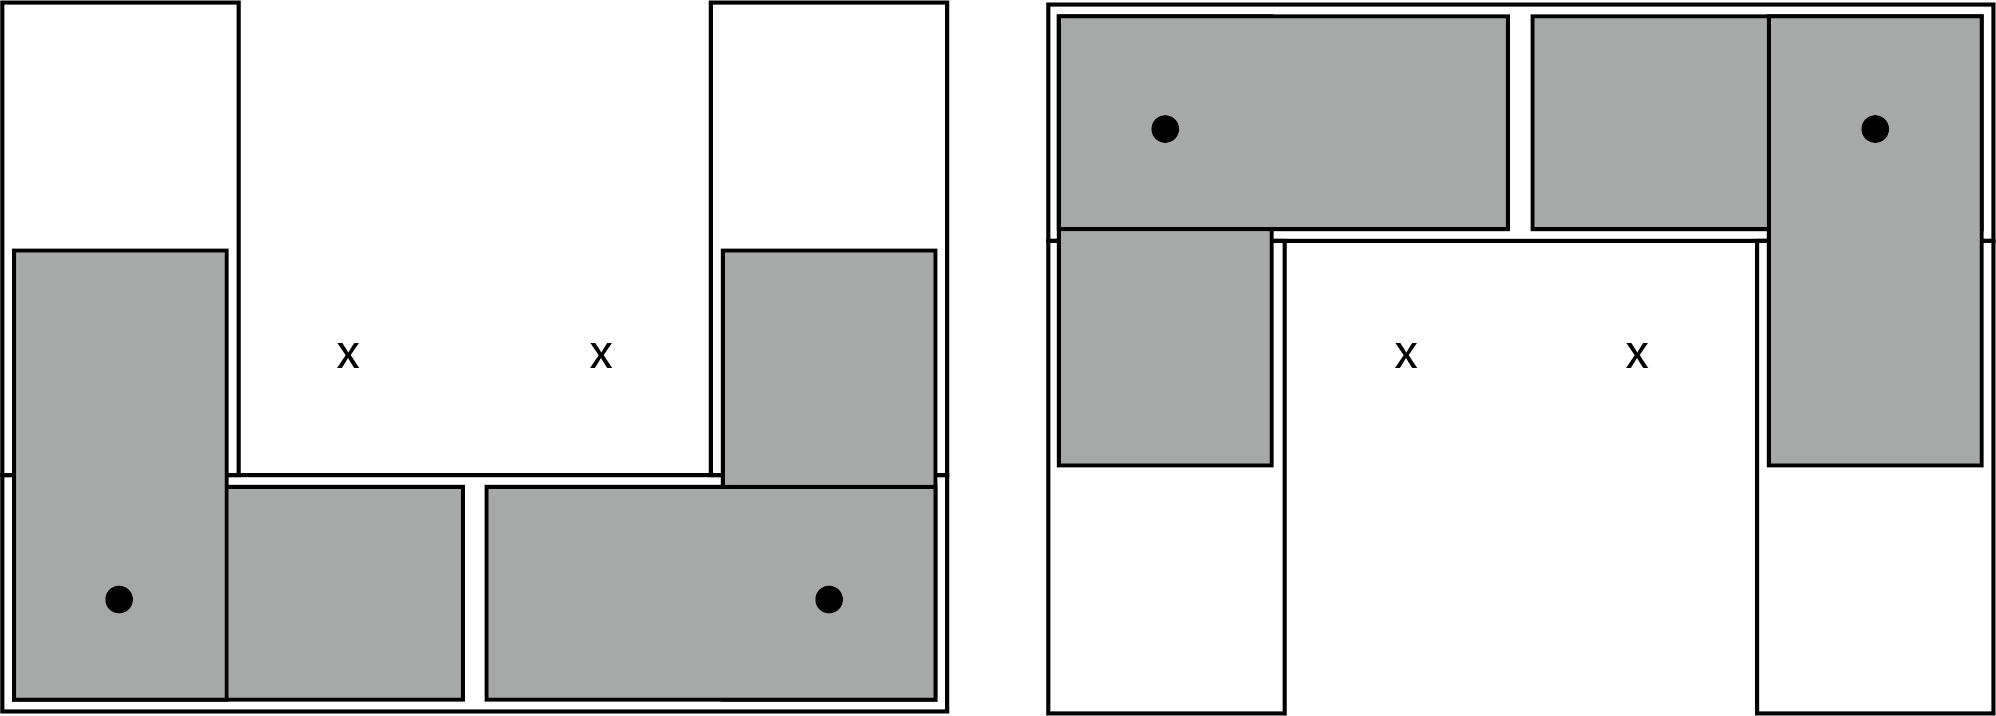
\includegraphics[width=0.9\columnwidth]{fig/Eckrotationen.png}
  \caption{Die vier Rotationsmöglichkeiten eines Eckbereichs.}\label{fig:real:eckrotationen}
\end{figure}
Um diese lokalen Eckrotationen zu berechnen wird für jede Ecke zunächst ein normierter Vektor in Richtung des Punktes x anhand der Mittelpunkte beider \textit{WallLayer} und dem Eckpunkt gebildet.
Dies entspricht sozusagen der \textit{Richtung} der Ecke.
Dieser Vektor wird dann um das Inverse der Rotation einer der am \textit{Corner} beteiligten \textit{WallLayerGroup} rotiert, um ihn in das globale Koordinatensystem zu überführen.
Durch diese Rotation ist nun die Achse der Ecke gleich der z-Achse des Koordinatensystems.
Deshalb kann mithilfe des Arkustangens der Quadrant herausgefunden werden, in dessen Richtung der Vektor zeigt.
Da sowohl bekannt ist, dass der Vektor des Punktes x um 45\degree{} zur eigentlichen Eckrotation versetzt ist, als auch, dass die Rotation nur die z-Achse betrifft, kann mit dem Ergebnis des Arkustangens nun ein Quaternion erstellt werden, welches die spezielle lokale Eckrotation beschreibt.
Auch mit T-Kreuzungen kann in ähnlicher Weise verfahren werden. 
Allerdings existieren hierbei statt vier nur zwei Fallunterscheidungen.

\paragraph*{Abschluss eines Wandstücks} Wandenden sind mithilfe der \textit{Corner} identifizierbar.
Existiert kein \textit{Corner} an einem Ende einer Schicht, handelt es sich entweder um ein Wandende oder den Außenbereich einer Öffnung.
Dank den Informationen in den einzelnen Schichten eines Wandstücks, können die durch den Verband an diesen Bereichen gebliebenen Lücken kleinere Bausteine eingefügt werden, sofern dies gewünscht ist.
Beispiele für aufgefüllte Wandenden sind in Abschnitt~\ref{concept:wandende} zu sehen.
Im Gegensatz dazu schließen die in Abbildung~\ref{fig:basics:verbaende} vorgeführten Wandstücke nicht mit verkleinerten Bausteinen ab.

\paragraph*{Besondere Bausteine über Öffnungen} Wird von einer Öffnung ein Sturz definiert, so muss dieser ähnlich zu einem Baustein des Standardmoduls ebenfalls in einen konkreten \textit{Brick} überführt werden.
Die lokale Position innerhalb des Wandstücks liefert die Öffnung selbst.
Die Dimensionen des Bausteins sind mithilfe des Moduls, das zur Beschreibung des Sturzes erstellt wurde, wie gewohnt vorgegeben.

\begin{figure}[hb]
  \centering
  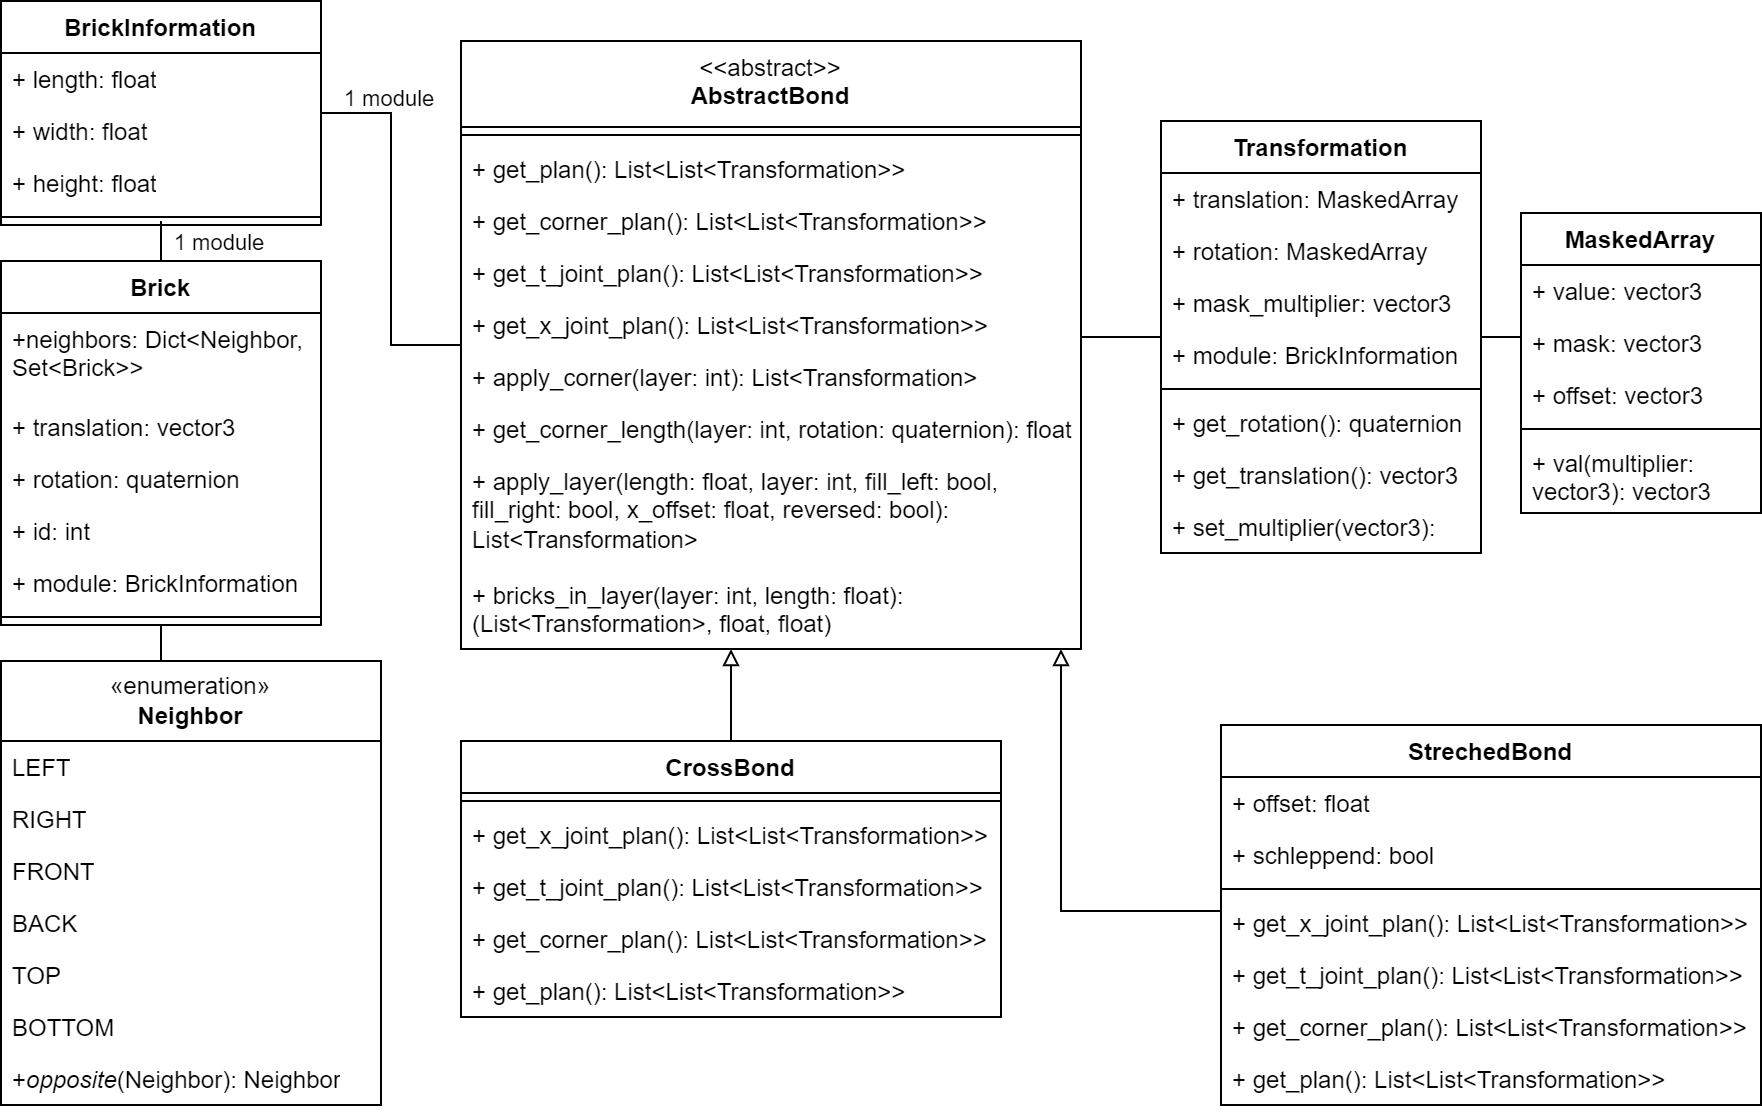
\includegraphics[width=0.9\columnwidth]{fig/klassendiagramm_bonds.drawio.png}
  \caption{Klassendiagramm für die Mauerwerksverbände.}\label{fig:real:class_diagram_bonds}
\end{figure}

\subsection{Nachbarschaftsbeziehungen zwischen Bausteinen}
\begin{figure}[h!bt]
  \begin{subfigure}[b]{0.49\columnwidth}
    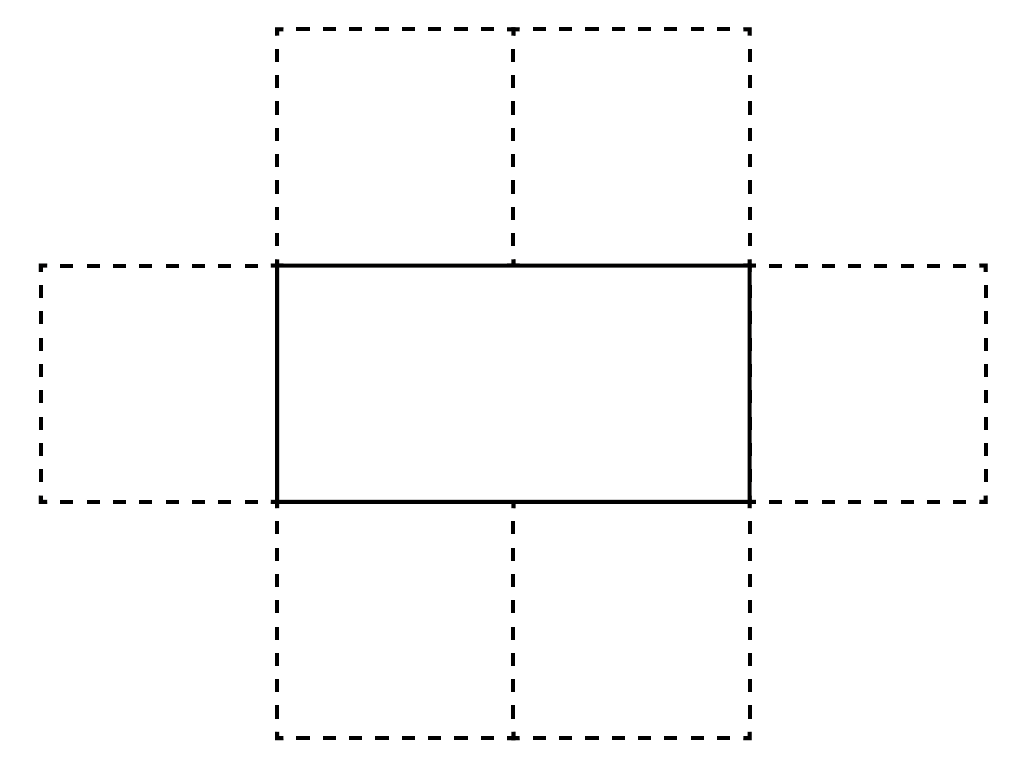
\includegraphics[width=\columnwidth]{fig/raster_neighbors1.png}
    \caption{Nachbarschaften in einem 1$\times$1 Raster}\label{fig:real:raster_neigbors1}
  \end{subfigure}
  \hfill
  \begin{subfigure}[b]{0.49\columnwidth}
    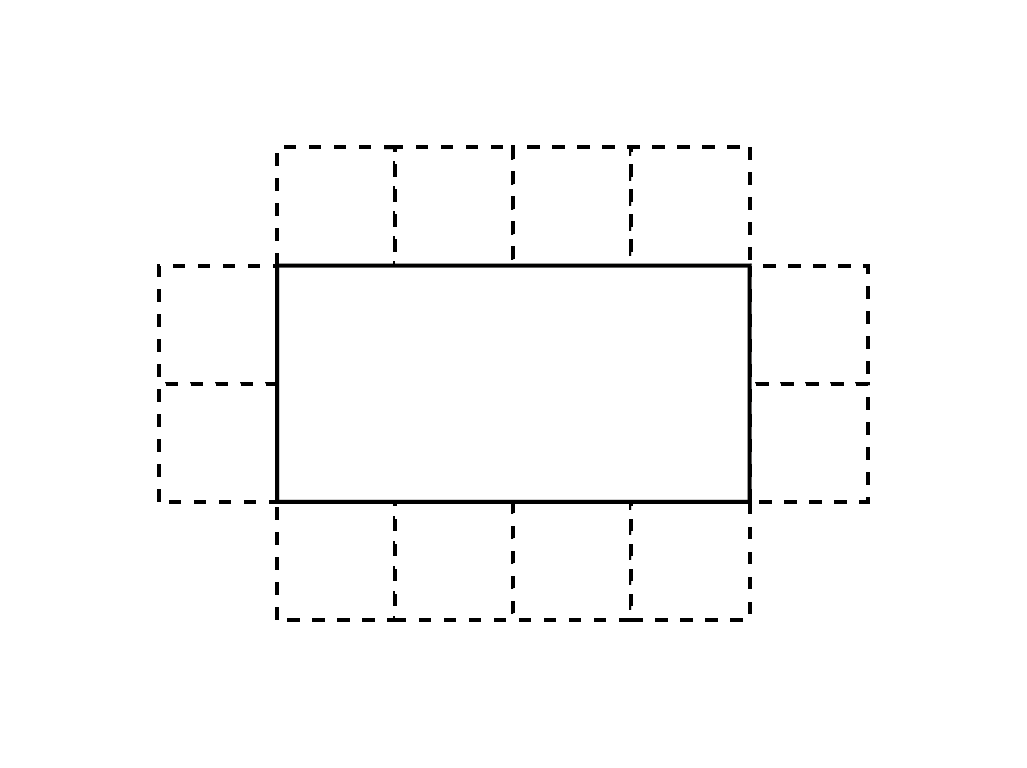
\includegraphics[width=\columnwidth]{fig/raster_neighbors2.png}
    \caption{Nachbarschaften in einem 0.5$\times$0.5 Raster}\label{fig:real:raster_neigbors2}
  \end{subfigure}
  \caption{Mögliche rasterabhängige Nachbarschaften.}\label{fig:real:raster_neigbors}
\end{figure}

Um valide Nachbarschaften zwischen den berechneten Bausteinen festzustellen, werden die den Wandstücken zugeordneten Raster herangezogen.
In Abbildung~\ref{fig:real:raster_neigbors} ist der Effekt zweier unterschiedlicher Raster auf den gleichen Baustein dargestellt.
Die gestrichelten Plätze sind potenzielle Nachbarfelder.
Da es sich allerdings nicht um eine zwei-, sondern eine dreidimensionale Umgebung handelt, gibt es auch unter- und oberhalb der Bausteine mögliche Nachbarn.
Um Bausteinen diese Informationen hinzuzufügen, wurde die Enumeration \textit{Neighbor} und das \textit{neighbors} Feld in der Klasse \textit{Brick} erstellt.
Dies ist im Klassendiagramm in Abbildung~\ref{fig:real:class_diagram_bonds} zu sehen.
Die Enumeration \textit{Neighbor} definiert sechs mögliche Nachbarschaftsarten: linke, rechte, vordere, hintere, darüber und darunter liegende Nachbarn.
Die Klasse \textit{Brick} wird mit dem Feld \textit{neighbors} um ein Dictionary ergänzt, welches zu jedem dieser Fälle eine Menge eindeutiger Bausteine beinhalten kann.
Der Grund dafür ist, dass es einem Baustein je nach Raster möglich ist etwa mehrere linke Nachbarn zu haben (siehe Abbildung~\ref{fig:real:raster_neigbors2}).
Nun kann für jeden Baustein durch den Vergleich mit allen anderen herausgefunden werden, welche Bausteine welche Nachbarfelder besetzen.
Über die Funktion \textit{opposite} der Enumeration \textit{Neighbor}, kann im selben Zug oftmals auch den gefundenen Bausteinen ein Nachbar hinzugefügt werden.
Das hängt allerdings von den lokalen Rotationen der Nachbarn ab.


\subsection{Export}\label{real:export}
In Kapitel~\ref{concept:regelbasierte_bauplandeduktion} wurde bereits erarbeitet, wie sich Regeln in einer Ontologie definieren lassen.
Gleichzeitig wurde die Klasse \textit{Brick} konzeptioniert, die alle notwendigen Informationen zu einem Baustein enthält, um diesen nach weiteren Eigenschaften zu analysieren.
Sämtliche Klassen und Eigenschaften des Konzepts aus diesem Kapitel konnten mithilfe des Ontologie-Editors Protégé (siehe Kapitel~\ref{basics:protege}) umgesetzt werden.
Dank der Python Bibliothek \textit{Owlready2} (siehe Kapitel~\ref{basics:owlready}) kann diese Ontologie leicht an den bisher entstandenen Programmcode angeschlossen werden.
Zunächst werden die in der Ontologie erstellten Regel-Individuen ausgelesen und während der Befüllung der Ontologie mit Brick-Instanzen auf deren Eigenschaften angewandt.
Insbesondere das Auffüllen der \textit{dependsOn}-Eigenschaft anhand der zuvor ausgerechneten Nachbarschaften spielt hierbei eine wichtige Rolle.
Owlready erlaubt das Wählen und Starten unterschiedlicher Reasoner.
Nachdem die Berechnungen des Reasoners beendet sind, kann über eine Anfrage, welche alle Individuen einer bestimmten Klasse zurückgibt, die derzeitige Liste platzierbarer Bausteine ausgelesen werden.
Da es in anderen Programmiersprachen womöglich schwieriger ist, Daten aus Ontologien auszulesen, werden zusätzlich alle relevanten Informationen zu den Bausteinen in einer sogenannten JSON-Datei zur Verfügung gestellt.
JSON (JavaScript Object Notation) ist ein weit verbreitetes, menschenlesbares Austauschformat, zu welchem in den meisten Programmiersprachen hilfreiche Bibliotheken existieren, die das Auslesen und Strukturieren von Daten aus diesen Dateien erleichtern~\cite{json}.
Um eine direkte und nutzerfreundliche Alternative zu textuellen Ausgaben anzubieten, werden außerdem noch 3D Meshes erzeugt und als STL-Dateien exportiert.
Dabei wird nicht nur ein einziges Mesh des gesamten Ergebnisses generiert, sondern auch von einigen wichtigen Zwischenergebnissen.
Diese Meshes lassen sich in einem beliebigen 3D Viewer leicht betrachten und auf Probleme untersuchen.
So können Fehler in der Modellierung oder in der Implementierung leichter erkannt werden.